\chapter{Discussion and further work}
Multiple aspects of the work presented in this report can be expanded upon.

\section{Torque estimation}
The current method for torque estimation, involving NN, seems promising based 
on results seen in other works \cite{wu_neural-network-enhanced_2019, 
toro-ossaba_myoelectric_2024}. However, the examples given and the models 
developed in this report are far from optimal.  

As previously stated, the models work rather well in the range of the training 
load but fail in experiments involving loads outside of that range, e.g. 
Figure \ref{fig:ovc10kg}. Whats more is that the models have a very noisy response 
that may cause user discomfort. A few ways to improve these results include: 

\begin{IEEEitemize}
\item Using different input parameters for the NN models
\item Improving the quality of the training data
\item Modifying the NN model architecture 
\item Smoothing the NN output
\end{IEEEitemize}

\bigskip

Different input parameters can consist in considering rotation speed and/or 
raw sEMG data, like Wu et al. \cite{wu_neural-network-enhanced_2019}, or 
taking triceps sEMG values into account, like \cite{toro-ossaba_myoelectric_2024}. 

\bigskip

The training data quality may be improved in a number of ways.  

Firstly, the equation used to calculate torque from angle data \ref{eq:torque} 
may be replaced by a more accurate method of gathering torque information. 
Indeed, the current model can not estimate torque unless there is movement, 
as illustrated in Figure \ref{fig:ovctoo_heavy}. Even though this is not part of 
the system's intended use cases it showcases that the torque calculation model is 
limited.  

Secondly, the way the current training data is used contains a sampling step 
where only one in 40 values is used. This makes the effective sampling rate 
of the training value to be equal to 40 times the sampling rate of the data, 
i.e. 40ms. However, the data sampling rate of the implemented sensor system is not 
the same, this must be one of the causes of the torque estimation's poor 
real-world performance. To fix this issue, either a new dataset must be created 
with this work's system, or the system's sampling rate must be calculated and 
used as the new effective sampling rate for NN training.  

Finally, more diverse experiment protocols may be considered.  

\bigskip

The current NN model architecture is based on the work of Toro-Ossaba et al. 
\cite{toro-ossaba_myoelectric_2024}. Similar sequential architectures with 
simply more layers, like those implemented by Lu et al. and Wu et al. 
\cite{lu_development_2019, wu_neural-network-enhanced_2019, wu_adaptive_2023} 
or ones using convolutional layers like shown by Zhang et al. 
\cite{zhang_physics-informed_2023} could be considered to improve estimation 
results. 

\bigskip

Lastly, multiple papers \cite{lu_development_2019, wu_neural-network-enhanced_2019, 
toro-ossaba_myoelectric_2024} use a Kalman filter to remove noise and smooth the 
estimated joint torque. This approach could be considered. 

\begin{figure}[htbp]
  \centering
  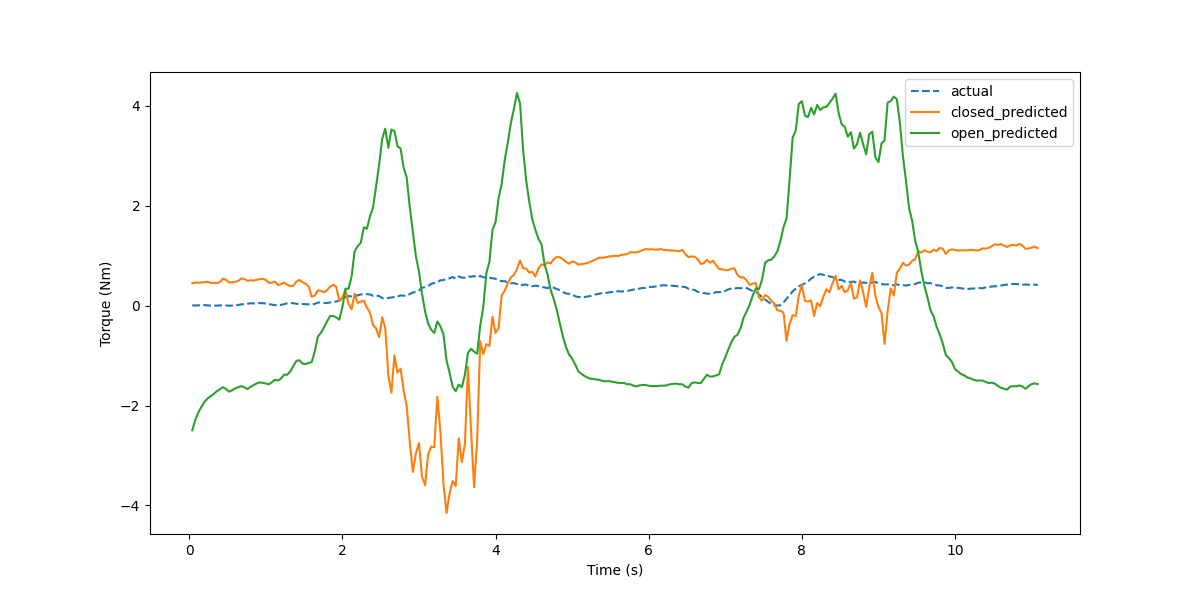
\includegraphics[width=0.8\linewidth]{open_vs_closed_too_heavy.png}
  \caption{Torque estimation for a weight that can not be lifted}
  \label{fig:ovctoo_heavy}
\end{figure}

\FloatBarrier
\section{Orthosis model}
A better model of the orthotic device can be used to improve the inverse model equation 
\eqref{eq:inv_model} and provide more accurate assistance. For starters, Lu et al. 
\cite{lu_development_2019} use a model that takes arm and forearm thickness into account. 
This could be a sufficient improvement over the current model. 

\FloatBarrier
\section{Control strategy}
As elementary components such as the torque estimation did not function properly 
during testing, the validity of the control strategy as a whole could not be 
determined. 
The current control strategy, inspired from the work of Toro-Ossaba et al. 
\cite{toro-ossaba_myoelectric_2024}, attempts to control the orthosis torque 
directly. As stated previously, other works \cite{lu_development_2019, 
wu_neural-network-enhanced_2019, wu_adaptive_2023} infer an angle delta from 
the torque estimation in order to use position control. This could be a possible 
progression path, but other options exist.  

One way of improving the control system is by integrating load estimation, 
possibly using an extended observer, to adjust the torque control to the 
carried load. 

Another way of continuing is by adding a model reference adaptive controller (MRAC) 
like in the work of Toro-Ossaba et al. \cite{toro-ossaba_myoelectric_2024}.  

Finally, a way of calculating the $K$ gain from Figure \ref{fig:control_diagram} 
with a high degree of fidelity, for a specified assistance level $\alpha$.  

\FloatBarrier
\section{Sensor system}
The implemented sensor system can be improved in a number of ways.  

The IMU sensors need to be fully calibrated before the beginning of each test, 
however a protocol that allows for quick calibration has not been found, 
and currently this calibration never finishes (for each sensor, at least one of 
the magnetometer, gyroscope, acceleration or system values does not achieve calibration). 
Therefore, the calibration loop has been commented out of the embedded code. 
Finding a calibration protocol or fixing the problem in another way could be 
beneficial to test results.  

As stated previously, the Myoware sensor is very sensitive to any electromagnetic 
noise that may affect it. Powering the sensor system with an external battery solved 
some of the encountered issues, but a cable connected to the ESP32's GND still 
had to be held by the user in order for the sEMG readings to be correct. 
Improving the reliability of these readings in all types of environments could 
lead to a safer and more usable system.  

Finally, a circuit board taking into account the possible addition of sensors can be 
designed for the sensor system.  

\FloatBarrier
\section{Main PC program}
The main python program linking the sensor system to the motor driver has an issue 
with BLE communication. The $Bleak$ python library used to establish and maintain 
the communication sometimes fails to connect to the $ESP32\_BLE\_server$ or 
disconnects abruptly for no apparent reason. Furthermore, whenever the communication 
is functional, the python program only manages to read the sensor values only about 
10 times per second, which is not enough for real-time applications. Fixing the BLE 
communication issues could greatly improve the reliability of the solution.

Lastly, $matplotlib.animation$ can be used to implement an equivalent to the 
Arduino IDE "Serial Monitor", in order to visualise data in real time even when 
working with BLE.  
\FloatBarrier
